\documentclass[11pt]{article}
\usepackage[utf8]{inputenc}
\usepackage[T1]{fontenc}
\usepackage{amsmath}
\usepackage{amsfonts}
\usepackage{amssymb}
\usepackage[version=4]{mhchem}
\usepackage{stmaryrd}
\usepackage{graphicx}
\usepackage[export]{adjustbox}
\graphicspath{ {./images/} }

\begin{document}
Investing in Portfolios of Single Hedge Funds

Although funds of funds provide instant diversification, they do so at the cost of an extra layer of fees. Whereas investors with a small amount to invest in hedge funds may find these fees to be cost-effective, larger investors need to compare the value of paying fees to funds of funds relative to building a portfolio of hedge funds using in-house resources.

There are a number of costs involved with the hedge fund due diligence process. It is expensive to subscribe to hedge fund databases, to hire and retain internal staff skilled in manager selection and portfolio construction, and to fund the expenses of visiting and evaluating each hedge fund manager. In addition, since the minimum investment in hedge funds tends to be rather large, only investors with very large portfolios can hold a diversified portfolio of hedge funds.

Keith Black discusses a buy-versus-build heuristic that institutional investors should consider. ${ }^{1}$ Keith H. Black (2004), Managing a Hedge Fund (New York: McGrawHill). Assume that a fund of funds approach has a second layer of hedge fund fees, including a management fee of $1 \%$ and an incentive fee of $10 \%$. Black estimates that a full internal program has a minimum annual cost of $\$ 1$ million for building and maintaining an internal fund evaluation program. Investors may find it costeffective to build their own hedge fund portfolio once assets allocated to hedge funds exceed $\$ 50$ million. This result is found by dividing $\$ 1$ million by $2 \%$, which is the total fee, assuming a typical incentive fee of $1 \%$ of AUM. However, for investors with less than $\$ 50$ million to invest in hedge funds, paying $2 \%$ fees to a fund of funds manager can be seen as a lower-cost alternative to spending $\$ 1$ million annually inhouse.

The next exhibit describes the minimum initial investment sizes required by individual hedge funds. The information presented in the exhibit can be used to help set an investment minimum for building an internal hedge fund portfolio. The median hedge fund has a minimum investment size of $\$ 500,000$. If investors need approximately 20 hedge funds to be well diversified, then investors would need a minimum hedge fund portfolio of $\$ 10$ million to consider investing directly in singlemanager hedge funds. Yet even if an investor has $\$ 10$ million to commit to hedge funds, the expenses of building the fund may be prohibitive (e.g., $\$ 1$ million of expenses, as discussed, would represent $10 \%$ of the $\$ 10$ million investment). Accordingly, small investors are attracted to funds of funds.

\begin{center}
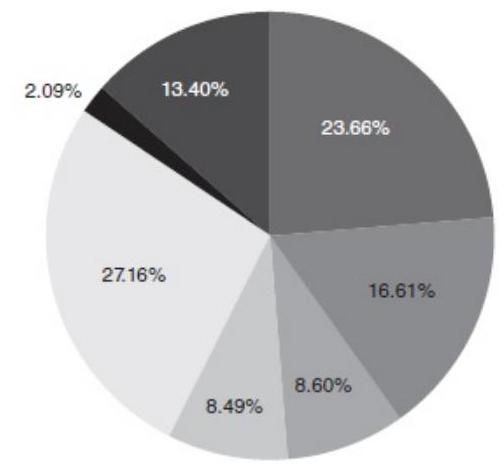
\includegraphics[max width=\textwidth]{2024_04_09_2a059f6740e65d00331bg-2}
\end{center}

\begin{center}
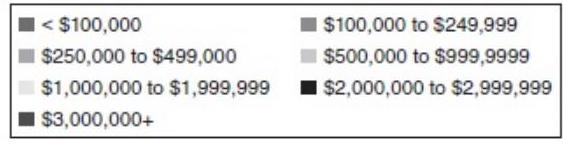
\includegraphics[max width=\textwidth]{2024_04_09_2a059f6740e65d00331bg-2(1)}
\end{center}

Minimum Investments Required by Hedge Funds, 4Q 2021


\end{document}